paragraph{Examples with Predication: }

Consider the following slightly more involved example than the first.

\begin{verbatim}

00	r2 <- r0 op r1
10	b_op r2, 030
20	r2 <- r3 op r0
30	r4 <- r2 op r0

\end{verbatim}

The time ordered execution sequence for this example is shown in
Figure~\ref{pex2}.

\begin{figure}
\centering
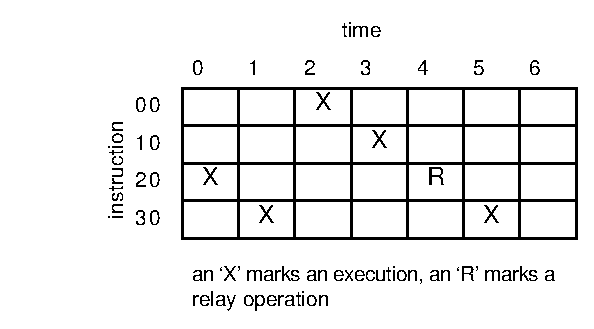
\epsfig{file=pex2.eps,width=2.50in}
\caption{{\em Timing of the code example, predication scenario 2.}
This example illustrates a relay operation that
can occur within an active station when a branch
predicate changes.
Execution of an instruction at a given time is
again indicated by an `X'.  A relay operation is indicated by an 'R'.}
\label{pex2}
\end{figure}

It is assumed that all instructions are loaded and that
the branch at 10 is initially predicted as not taken.
Since instruction 20 is not restricted from executing
due to the initial branch prediction of instruction 10,
it can execute immediately upon being loaded.
It is assumed that it does execute immediately and before
all other instruction shown.
Since instruction 30 is data dependent on instruction 20
when the branch is not taken, it snarfs up the
newly created value for register
{\tt r2}
from instruction 20 and is enabled to execute.
Instruction 30 gets to execute in the follow clock cycle.
Now, later, instruction 00 executes creating a new value for
register
{\tt r2}.
We assume that this is still a speculative value.
Note that since instruction 30 has already snarfed a value for
register
{\tt r2}
later in time than that created by instruction 00, it is not
enabled for execution due to this change.
Instruction 10, however, is data dependent on instruction 00 (through
{\tt r2})
and is enabled to execute.  
Note carefully also, that instruction 20 was snooping for both
its inputs and its output (register
{\tt r2}).  It had to snoop for newly created values for
{\tt r2}) in case it was determined that the execution the instruction
was squashed.  The new value of
register
{\tt r2} will be snarfed by instruction 20 from 
the output forward broadcast of
instruction 00.

Instruction 10, the branch now executes.
We now assume that after the branch at 10 executes, its output
predicate changes, that is, the branch is now predicted to
be taken.  Its output predicate is broadcast and
instruction 20, snooping on the branch output predicate,
sees the broadcast and snarfs it.  Instruction 20, now has
an indication that its assignment of its executed value
is no longer valid and instead broadcasts its relayed value
for register
{\tt r2}.
Finally, this newly broadcast value for
register
{\tt r2} will
be snarfed by instruction 30 enabling it to re-execute also.
Finally instruction 30 executes in clock cycle 5 as shown in the
figure above.

This example showed how the effects of instructions within the
domain of a branch are squashed when the branch either
changes to a prediction of taken or is resolved to be taken.
It also showed how the incorrect results of instructions beyond the
join of a branch are corrected when a branch outcome is changed.
